\chapter{A Framework for Robot Programming}\label{sec:Contribution}

\cite{ingrand2017deliberation} identifies six deliberation functions that are necessary to interface with robotic system to act autonomously: planning, acting, monitoring, observing, learning, and goal reasoning (\fig{fig:deliberationfunctions}).

\begin{figure}[h]
	\centering
	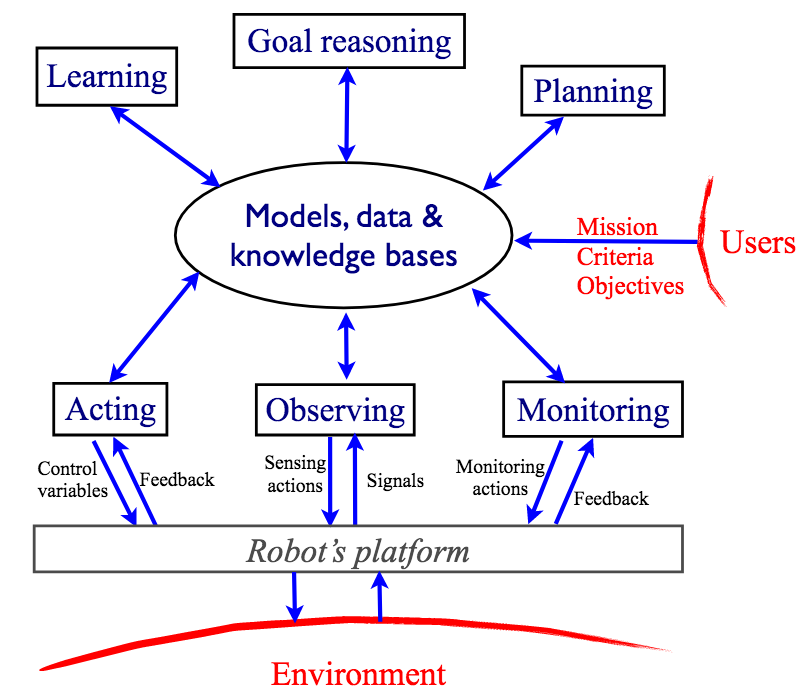
\includegraphics[scale=0.50]{figures/deliberationfunctions}
	\caption{Schematic view of deliberation functions \cite{ingrand2017deliberation}}
	\label{fig:deliberationfunctions}
\end{figure}

The framework that we propose with this project allows users without any programming knowledge to teach a robot a goal-oriented behaviour. 
Unlike current PbD implementations, which teach the robot an action sequence to achieve a goal, we want to equip the robot with all actions required to generate the action sequence autonomously using automated planning techniques. The user needs to construct a planning domain, consisting of all actions that the user taught the robot by demonstration.
 Using this knowledge base, the user can define a planning problem, for which the robot will generate a plan.
 PbD implementations using Hidden Markov Models recognise examples from training sets and use probabilities to assign an action.
 This requires training sets that are large enough to cover a wide range of possible world states.
 With our goal-oriented approach, the robot can solve an infinite number of goals, by using a limited set of actions.
 Figure \ref{fig:framework} shows the layout of our proposed framework (user activities are shown in blue and robot activities are shown in red).
 

  \begin{figure}[!h]
    \centering
    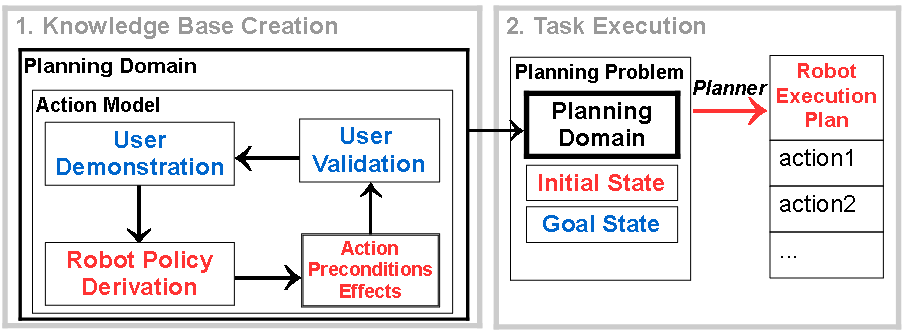
\includegraphics[scale=0.66]{figures/framework2}
    \caption{Framework for Robot Programming by Demonstration}
    \label{fig:framework}
  \end{figure}

\section{Creation of the Knowledge Base}
The user (in blue) interacts with the robot (in red) using a graphical interface.
The user has to create the planning domain, as specified in \sect{subsec:Planning domain description}, by defining the requirements, object types and predicates, i.e. conditions that can be included in the action definition.
The graphical interface should present the PDDL definitions in English sentences for the user.
Note that the object type definition at this stage is only at a syntactical level.
The instantiation of the locations and objects only occurs in the problem definition.
This leaves the user with the creation of the action models.

The actions will be created sequentially by iteratively providing demonstrations of the each individual action.
The robot extracts the relevant information from the demonstration using its sensors and builds a model of the learned skill.
By observing the changes in the state of the world, the robot suggests preconditions and effects, selected from the domain description, to be associated with the taught action.
After each demonstration, the user is presented with options to reproduce the learned skill or to modify the observed conditions.
The user either validates the learned action or provides another demonstration to refine it.
 

The action can be learned by generalising over a set of trajectories and by using statistical learning techniques, to deal with uncertainty contained in multiple motion demonstrations \cite{ude1993trajectory}.
Once the user is confident about the created action model and its associated conditions, they can save it to the knowledge base.
 This process is repeated for all action models that are required to build the knowledge base for the complex task.
 The action models are automatically translated into PDDL, allowing the creation of a PDDL domain, without the requirement for any programming knowledge.

\section{Task Execution}
The created knowledge base is internally connected with a planner.
 The user needs to create a planning problem, as specified in \sect{subsec:PPDescription}, by listing all objects of the planning problem.
 To associate the PDDL objects with the physical objects in the real world, the user needs to assign features to each object in the planning problem, to allow their easy recognition.
 For instance, the robot can learn to recognise objects by their colour or shape, and locations can be saved using their end effector coordinates.

Instead of defining the initial state, the robot should recognise it using its sensors, allowing the user to verify the robot's learned object recognition.
 Once the planning problem has been defined, the robot can generate a plan.
 The action sequence will then be executed by the robot in order to achieve the goal state.
 If the user changes the goal, a new plan will be generated accordingly.
This removes the intermediate step of having to define an action sequence manually every time the goal changes.
 
If the proposed solution is not optimal, the user can modify them or refine the action models.
 Missing predicates in the action definition can lead to suboptimal solutions.
 The generation of an action sequence provides the user with the opportunity to test the soundness of their created action models.\\

\noindent In summary, our proposed framework links techniques from the two disciplines Programming by Demonstration and Automated Planning to create a means for the non-expert user to teach a robot a goal-oriented behaviour.
 The user's steps can be summarised as follows:

\begin{enumerate}
\item Define the requirements, types and predicates for the domain description.
\item For all actions:
\begin{enumerate}
\item Record an action demonstration for the robot learner.
\item Verify the derived policy and validate the proposed preconditions and effects.
\item Optionally provide additional demonstrations to refine action.
\end{enumerate}
\item Define a planning problem using the created domain, including a goal state.
\item \textit{The robot recognises the initial state and generates a plan.}
\item Verify that the action sequence of the plan is correct.
\item Optionally refine the created action models.
\end{enumerate}